%%%%%%%%%%%%%%%%%%%%%%%%%%%%%%%%%%%%%%%%%
% Short Sectioned Assignment LaTeX Template Version 1.0 (5/5/12)
% This template has been downloaded from: http://www.LaTeXTemplates.com
% Original author:  Frits Wenneker (http://www.howtotex.com)
% License: CC BY-NC-SA 3.0 (http://creativecommons.org/licenses/by-nc-sa/3.0/)
%%%%%%%%%%%%%%%%%%%%%%%%%%%%%%%%%%%%%%%%%

%----------------------------------------------------------------------------------------
%	PACKAGES AND OTHER DOCUMENT CONFIGURATIONS
%----------------------------------------------------------------------------------------

\documentclass[paper=a4, fontsize=11pt]{scrartcl} % A4 paper and 11pt font size

% ---- Entrada y salida de texto -----

\usepackage[T1]{fontenc} % Use 8-bit encoding that has 256 glyphs
\usepackage[utf8]{inputenc}
\usepackage{fourier} % Use the Adobe Utopia font for the document - comment this line to return to the LaTeX default

% ---- Idioma --------

\usepackage[spanish, es-tabla]{babel} % Selecciona el español para palabras introducidas automáticamente, p.ej. "septiembre" en la fecha y especifica que se use la palabra Tabla en vez de Cuadro

% ---- Otros paquetes ----

\usepackage{url} % ,href} %para incluir URLs e hipervínculos dentro del texto (aunque hay que instalar href)
\usepackage{amsmath,amsfonts,amsthm} % Math packages
%\usepackage{graphics,graphicx, floatrow} %para incluir imágenes y notas en las imágenes
\usepackage{graphics,graphicx, float} %para incluir imágenes y colocarlas
\usepackage{epstopdf}
\usepackage[gen]{eurosym} %para incluir el símbolo del euro
\usepackage{cite} %para incluir citas del archivo <nombre>.bib
%\graphicspath{/images}

% Para hacer tablas comlejas
%\usepackage{multirow}
%\usepackage{threeparttable}

%\usepackage{sectsty} % Allows customizing section commands
%\allsectionsfont{\centering \normalfont\scshape} % Make all sections centered, the default font and small caps

\usepackage{fancyhdr} % Custom headers and footers
\pagestyle{fancyplain} % Makes all pages in the document conform to the custom headers and footers
\fancyhead{} % No page header - if you want one, create it in the same way as the footers below
\fancyfoot[L]{} % Empty left footer
\fancyfoot[C]{} % Empty center footer
\fancyfoot[R]{\thepage} % Page numbering for right footer
\renewcommand{\headrulewidth}{0pt} % Remove header underlines
\renewcommand{\footrulewidth}{0pt} % Remove footer underlines
\setlength{\headheight}{13.6pt} % Customize the height of the header

\numberwithin{equation}{section} % Number equations within sections (i.e. 1.1, 1.2, 2.1, 2.2 instead of 1, 2, 3, 4)
\numberwithin{figure}{section} % Number figures within sections (i.e. 1.1, 1.2, 2.1, 2.2 instead of 1, 2, 3, 4)
\numberwithin{table}{section} % Number tables within sections (i.e. 1.1, 1.2, 2.1, 2.2 instead of 1, 2, 3, 4)

\setlength\parindent{0pt} % Removes all indentation from paragraphs - comment this line for an assignment with lots of text

\newcommand{\horrule}[1]{\rule{\linewidth}{#1}} % Create horizontal rule command with 1 argument of height


%----------------------------------------------------------------------------------------
%	TÍTULO Y DATOS DEL ALUMNO
%----------------------------------------------------------------------------------------

\title{	
\normalfont \normalsize 
\textsc{\textbf{Ingeniería de Servidores (2016-2017)} \\ Grado en Ingeniería Informática \\ Universidad de Granada} \\ [25pt] % Your university, school and/or department name(s)
\horrule{0.5pt} \\[0.4cm] % Thin top horizontal rule
\huge Memoria Práctica 1 \\ % The assignment title
\horrule{2pt} \\[0.5cm] % Thick bottom horizontal rule
}

\author{Nombre Apellido1 Apellido2} % Nombre y apellidos

\date{\normalsize\today} % Incluye la fecha actual

%----------------------------------------------------------------------------------------
% DOCUMENTO
%----------------------------------------------------------------------------------------

\begin{document}

\maketitle % Muestra el Título

\newpage %inserta un salto de página

\tableofcontents % para generar el índice de contenidos

\listoffigures

\listoftables

\newpage

\textbf{NOTA: en caso de problema al compilar, compruebe que tiene el paquete: texlive-babel-spanish.noarch }  \\
 
 
Editores recomendados:
\begin{itemize}
\item TexStudio 
\item Gummi 
\item Texmaker 
\item Kile 
\item WinEdt 
\item Emacs 
\item Vim 
\end{itemize}

aunque existen muchos más...\\

Recomendación: si tiene algún problema, siempre puede consultar el registro de compilación (\textit{nombrearchivo}.log)donde se le indicará qué problema hay en el documento.

\newpage

%----------------------------------------------------------------------------------------
%	Cuestión 1
%----------------------------------------------------------------------------------------

\section{Escribir aquí el enunciado de la cuestión}

Cada etiqueta va precedida de la barra invertida \textbackslash , por ejemplo, para diferenciar las secciones correspondientes a cada cuestión, usaremos \textbackslash section. 

\LaTeX es popular por permitir escribir ecuaciones de una manera rápida y sencilla, p.ej.

\begin{align} 
\begin{split}
(x+y)^3 	&= (x+y)^2(x+y)\\
&=(x^2+2xy+y^2)(x+y)\\
&=(x^3+2x^2y+xy^2) + (x^2y+2xy^2+y^3)\\
&=x^3+3x^2y+3xy^2+y^3
\end{split}					
\end{align}

Ejemplo de cómo escribir matrices
\begin{align}
A = 
\begin{bmatrix}
A_{11} & A_{21} \\
A_{21} & A_{22}
\end{bmatrix}
\end{align}

Ejemplo de la inserción de una matriz, fíjese en cómo hay que introducir un \& entre cada columna y dos barras invertidas ( \textbackslash\textbackslash ) al final de cada fila.


%------------------------------------------------

\subsection{enunciado de una subcuestión}

Para contestar a preguntas concretas dentro de una cuestión, puede usar la etiqueta \textbackslash subsection.

También puede anidar más niveles usando \textbf{subsubsection} y \textbf{paragraph}



%----------------------------------------------------------------------------------------
%	Cuestión 2
%----------------------------------------------------------------------------------------

\section{Ejemplos de listas de elementos}

usaremos la etiqueta \textbackslash itemize y  \textbackslash enumerate para las listas de elementos y listas enumeradas. Fíjese en que se pueden anidar.

%------------------------------------------------

\subsection{Ejemplo de cómo usar listas de elementos (items) anidados}
\begin{itemize}
	\item First item in a list 
		\begin{itemize}
		\item First item in a list 
			\begin{itemize}
			\item First item in a list 
			\item Second item in a list 
			\end{itemize}
		\item Second item in a list 
		\end{itemize}
	\item Second item in a list 
\end{itemize}

%------------------------------------------------

\subsection{Ejemplo de una lista numerada}
\begin{enumerate}
\item First item in a list 
\item Second item in a list 
\item Third item in a list
\end{enumerate}

%----------------------------------------------------------------------------------------


%----------------------------------------------------------------------------------------
%	Cuestión 3
%----------------------------------------------------------------------------------------

\section{Incluyendo figuras en el texto}

%------------------------------------------------

Vamos ver cómo a incluir alguna figura en el documento y cómo citar la fuente de donde se ha cogido. Hay que asegurarse de que es posible reutilizar la imagen observando con qué licencia está publicada, por defecto, todas tienen \copyright . En el buscador de imágenes de Google hay una opción que permite filtrar los resultados en base a las licencias de uso.

Para incluir las figuras usaremos la etiqueta \textbackslash figure y añadiremos [h, t ó b] para obligar a que la figura esté donde deseemos [here, top o bottom]. Cuando [h] no surta efecto y siga moviendo la figura de sitio deberemos usar [H]. Además, podemos incluir una descripción usando \textbackslash caption. Gracias a la etiqueta \textbackslash label podemos poner un nombre a la figura de modo que podamos hacer referencia a ésta usando la etiqueta \textbackslash ref . Por ejemplo, aquí estamos haciendo referencia a la Figura \ref{fig:figura1}. Es importante que la etiqueta esté siempre definida después de la descripción (\textbackslash label siempre después de  \textbackslash caption). 

\begin{figure}[H] %con el [H] le obligamos a situar aquí la figura
\centering
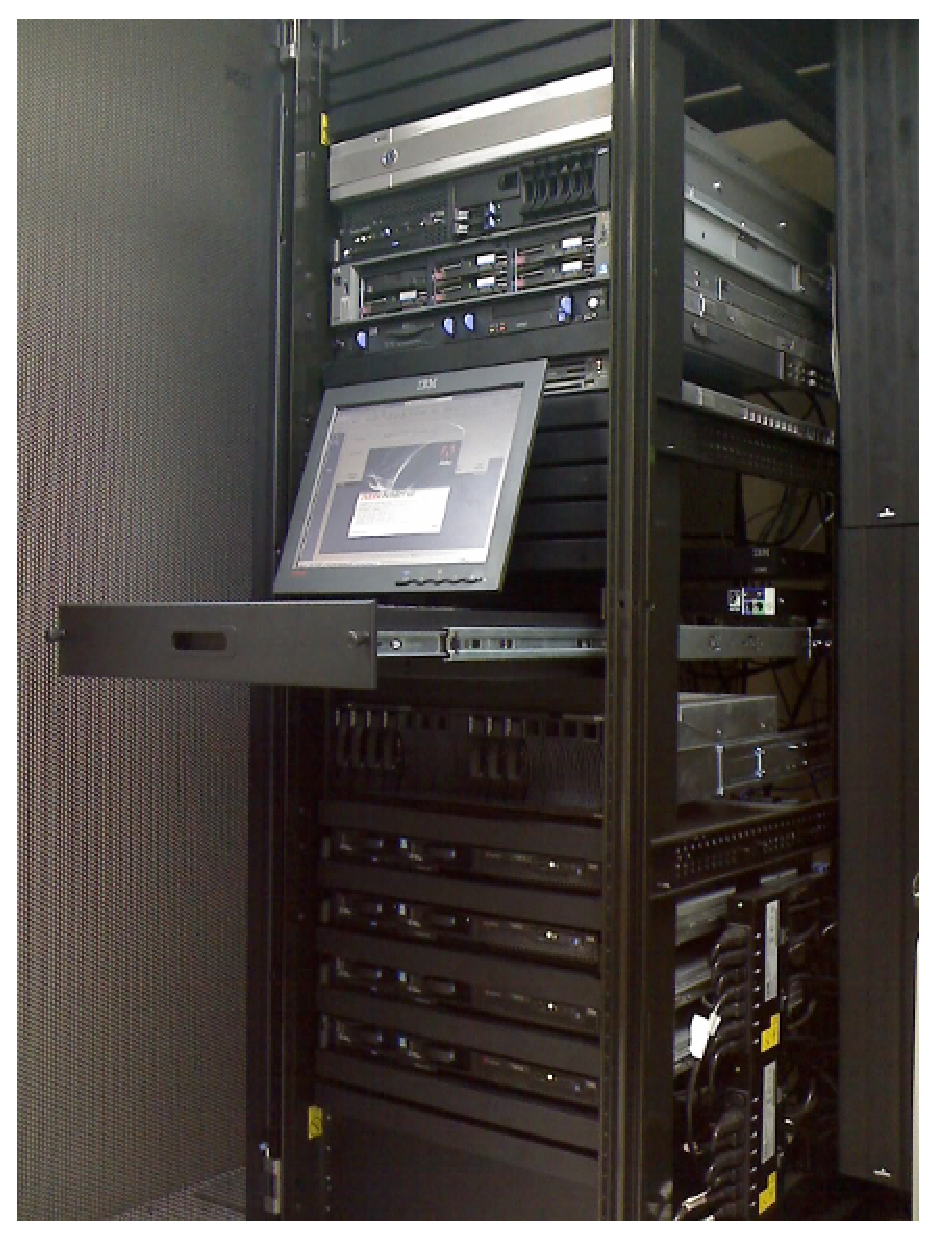
\includegraphics[scale=0.5]{Figura1.eps}  %el parámetro scale permite agrandar o achicar la imagen. En el nombre de archivo puede especificar directorios
\caption{Este es un ejemplo de cómo insertar una figura y citar la fuente con la etiqueta \textbackslash cite :  \cite{figura1} (para añadir la nota a pie de figura es necesario instalar un paquete extra, consulte el registro de compilación cuando tenga algún problema)} \label{fig:figura1}
\end{figure}

%------------------------------------------------

%----------------------------------------------------------------------------------------
%	Cuestión 4
%----------------------------------------------------------------------------------------

\section{Mostrando tablas}

%------------------------------------------------

Por último aquí tiene un ejemplo de una tabla sencilla (Tabla \ref{tab:tablasencilla} debe usar la etiqueta \textbf{table} y luego \textbf{tabular} especificando el número de columnas así como la posición del texto dentro de ellas (r,c o l para derecha, centro o izquierda respectivamente).

Con la etiqueta \textbackslash hline trazará líneas horizontales y, al igual que con las figuras, debe especificar [H] para que sitúe la tabla justo debajo (a continuación) y puede etiquetar la tabla con \textbackslash label y su descripción con \textbackslash caption.

%----------------Tabla sencilla--------------------------------
\begin{table}[H]
\centering
\begin{tabular}{|c|c|c|}
\hline
\textbf{ Etiqueta1} & \textbf{Valor1} & \textbf{Valor2} \\
\hline
Coche & amarillo & 37,5\% \\
Moto & azul & 55\% \\
\hline
\end{tabular}  
\caption{Ejemplo de una tabla sencilla} \label{tab:tablasencilla}
\end{table}


%----------------------------------------------------------------------------------------
%	Cuestión 5
%----------------------------------------------------------------------------------------

\section{Incluyendo las referencias}

A lo largo del texto, tendrá que incluir referencias, para ello puede usar las notas a pie de página con \textbackslash footnote \footnote{Este es un ejemplo} o añadiendo citas con \textbackslash cite \cite{mrx05,prueba2}. \LaTeX puede gestionar las referencias mediante BibTex, que genera entradas bbl a partir de un archivo .bib. También puede incluirlas directamente en el documento fuente como entradas dentro de una sección (thebibliography) dentro del mismo documento (son las generadas en el archivo .bbl por BibTex). No obstante, se recomienda el uso del archivo .bib como buena práctica a seguir cuando se trabaje con \LaTeX.

Para incluir las referencias usaremos la etiqueta \textbackslash bibliography especificando su estilo: \textbackslash bibliographystyle que, en nuestro caso, es plain. Una duda muy común es el orden o desorden en la numeración automática que reciben las referencias, si quiere que se numeren según vayan apareciendo pruebe con otro estilo (p.ej. ieeetr o apalike)

Si va a incluir un URI o una URL es recomendable que use la etiqueta \textbackslash url para "escapar" de los caracteres reservados de una manera cómoda. Otra forma de "escapar" es utilizando la etiqueta \textbackslash verbatim , p.ej. 

\begin{verbatim}
Cualquier texto que incluya _ % { } , etc. sin tener que usar \ para escribirlo.
\end{verbatim}



%------------------------------------------------

\bibliography{citas} %archivo citas.bib que contiene las entradas 
\bibliographystyle{plain} % hay varias formas de citar

\end{document}
